\documentclass[a4paper, 12pt, twoside]{article}
\usepackage[utf8]{inputenc}
\usepackage[english, italian]{babel}
\usepackage[a4paper,left=2cm,right=2cm,top=2.5cm,bottom=2.5cm]{geometry}

% Pacchetti
\usepackage{graphicx}
\usepackage{hyperref}
\usepackage[ruled, vlined]{algorithm2e}
\renewcommand{\thealgocf}{}
\usepackage[T1]{fontenc}
\usepackage{amsmath}
\graphicspath{ {./images/} }
\linespread{0.9}


\title{Primo Progetto di Social Computing}
\author{Massimiliano Baldo 142296\\
        Simone Dalla Pietà 141995\\
        Ilaria Fenos 142494\\
        Emanuele Lena 142411
        }
\date{A.A. 2020/21}




% -------------------------------------------------------------------------------- %
% ------------------------------- INIZIO DOCUMENTO ------------------------------- %
% -------------------------------------------------------------------------------- %
\begin{document}

\maketitle
% -------------------------------------------------------------------------------- %
% ------------------------------- INDICE CONTENUTI ------------------------------- %
% -------------------------------------------------------------------------------- %
\tableofcontents
\thispagestyle{empty}  % Sta roba serve a far cominciare la numerazione delle pagine
\newpage               % a partire dalla pagina successiva (dell'Introduzione)
\setcounter{page}{1}   %

% -------------------------------------------------------------------------------- %
% ------------------------------- INTRODUZIONE ------------------------------- %
% -------------------------------------------------------------------------------- %
\section{Introduzione} \label{sec:intro}


\subsection{Obiettivi del progetto}
L’obiettivo del progetto è di reperire una porzione della rete sociale del social network  Twitter, per poi fare un’analisi applicando alcune delle più tipiche tecniche di studio dei grafi. \\*
Nel dettaglio, si intende:
\begin{itemize}
    \item Reperire i dati pubblici di 5 di profili di partenza, dei profili a loro direttamente correlati (followers e followed) e di ulteriori profili casuali (scelti secondo certi criteri spiegati in seguito)
    \item Costruire un grafo che rappresenta la rete sociale, dove
    \begin{itemize}
        \item i nodi sono i profili scaricati
        \item gli archi (diretti) indicano una relazione di follower → following (“chi segue chi”)
    \end{itemize}
    \item Applicare le più comuni tecniche di analisi sul grafo, quali la visualizzazione del grafo, misura delle distanze e centralità, calcolo della copertura minima e la stima della “small-world-ness” del grafo.
\item Calcolo delle correlazioni tra le variabili calcolate
\end{itemize} % :(

\subsection{Strumenti e tecnologie}
Si usano i seguenti strumenti e tecnologie:
\begin{itemize}
    \item API di Twitter - per il reperimento dei dati necessari
    \item Linguaggio Python - per la semplicità d’uso 
    \item Librerie (principali) del linguaggio Python: Tweepy, NetworkX, Pandas, Pyvis
    \item Strutture di supporto Cloud: Google Colaboratory per il codice e Google Drive per il salvataggio dei dati
\end{itemize}

% -------------------------------------------------------------------------------- %
% ----------------------- DOWNLOAD UTENTI E CREAZIONE GRAFO----------------------- %
% -------------------------------------------------------------------------------- %
\section{Reperimento dei dati} \label{sec:reperimento_dati}


\subsection{Metodologie di reperimento, rappresentazione e divisione del carico di lavoro}

\subsubsection{Metodologie di reperimento}
Il reperimento dei dati è stato effettuato tramite l’interrogazione degli endpoint di Twitter con il supporto della libreria Tweepy. Alcune funzioni vengono eseguite con il supporto di Cursor (strumento di Tweepy che gestisce automaticamente la paginazione dei risultati).

\subsubsection{Metodologie di rappresentazione}
Si è scelto di rappresentare i dati reperiti mediante dei dataframe Pandas. 
Nel dettaglio, le informazioni sono state rappresentate tramite questi due formati:
\begin{itemize}
    \item Il primo formato - d’ora in poi chiamato “df\_users” - rappresenta i dati dei singoli profili, un profilo per riga; ogni colonna corrisponde ad un campo dell’oggetto ritornato da api.get\_user, per esempio:
    \begin{itemize}
        \item la colonna “id” contiene il codice identificativo univoco del profilo,
        \item la colonna “screen\_name” contiene l’username (univoco) del profilo,
        \item la colonna “followers\_count” contiene il numero di seguaci (“followers”) del profilo;
    \end{itemize}
    \item Il secondo formato - d’ora in poi chiamato “df\_relations” - rappresenta tutte le relazioni di tipo “Follower segue Following” rilevate durante l’esplorazione.
    \begin{itemize}
        \item ogni riga indica una relazione del tipo “A segue B”;
        \item le colonne “Follower” e “Following” rappresentano rispettivamente i profili “che seguono” e “quelli seguiti”; ogni profilo si identifica con il suo id.
    \end{itemize}
\end{itemize}
A questi due formati principali si aggiunge un terzo formato - d’ora in poi chiamato “df\_accurate\_ relations” - utile a rappresentare i risultati delle interrogazioni effettuate con api.show\_friendship.
\begin{itemize}
    \item Ogni riga riporta i dettagli della relazione tra 2 profili (“source” e “target”)
    \item Oltre alle colonne “source” e “target”, ci sono altre 2 colonne “follow” e “followed \_by”, che indicano  rispettivamente se “source” segue “target” e se “source” è seguito da “target”.
\end{itemize}
Tutti questi dataframe sono stati salvati come dataset csv su una cartella Drive.

\subsubsection{Divisione del carico di lavoro}
Viste le limitazioni di interrogazioni effettuabili tramite le API di twitter, si è diviso il carico di lavoro delle interrogazioni su 4 notebook Colaboratory differenti, che - con lo stesso codice -  interrogano gli endpoint con chiavi d’accesso differenti in parallelo. \\* \\*
Ogni notebook ha quindi generato più datasets df\_users e df\_relations. Questi datasets sono stati poi uniti in un 2 unici datasets finali attraverso un opportuno codice che concatena i dataset e rimuove eventuali duplicati. \\* \\*
Si sono salvati i due dataset finali df\_users e df\_relations, sempre nel formato csv.


\subsection{Reperimento dei profili principali e dei profili direttamente connessi} 
Si è partiti dal reperimento dei dati di 5 profili principali. Di questi profili si sono reperiti tutti i dati pubblici con la chiamata di api.get\_user. Dopo di che, si sono reperiti anche i dati dei loro follower e following tramite le chiamate api.followers e api.friends. Durante il reperimento dei dati di followers e followed, si riempie anche il dataframe df\_relations con le informazioni su che relazione hanno quest’ultimi con il profilo principale:
\begin{itemize}
    \item Se un profilo A è follower del profilo principale X, si inserirà una riga “A segue X”;
    \item Se un profilo B è followed (friend) di X, si inserirà una riga “X segue B”.
\end{itemize}
5 profili principali:    @mizzaro, @damiano10, @Miccighel\_, @eglu81, @KevinRoitero


\subsection{Reperimento dei profili casuali aggiuntivi}
Per ognuno dei 5 profili principali, si scelgono 5 followers e 5 followed casuali. Come criterio di scelta, si considerano solo i followers con almeno 10 followers e i followed con almeno 10 followed (i profili si trovano cercando nel dataframe df\_relations). \\* \\*
Per ognuno dei 5 followers casuali si reperiscono gli ids dei suoi followers con  api.followers\_ids. Di questi ids, si scelgono casualmente 10, si recuperano i dati dei profili con tali ids (tramite  api.get\_user) e si annota su df\_relations di chi sono followers. \\* \\*
Si effettua una procedura analoga per i 5 followed casuali scelti e 10 loro followed casuali.


\subsection{Verifica della relazione tra i profili}
Si vuole verificare la relazione tra tutti i profili scaricati e i 5 iniziali. Per verificare la relazione, si chiama la funzione api.show\_friendship tra ognuno dei profili ed ognuno dei 5 iniziali (prendendo le opportune precauzioni per non verificare 2 volte la stessa relazione o verificare la relazione del profilo con se stesso). Viste le limitazioni di richieste sugli endpoint, confrontare tutti i profili sarebbe risultato molto dispendioso.

Si è giunti però alla conclusione, che già si conoscono le relazioni con i 5 profili iniziali:
\begin{itemize}
    \item Se un profilo è follower di uno dei 5, si individua durante la chiamata api.followers;
    \item Se un profilo è invece seguito da uno dei 5, si individua durante la chiamata api.friends
\end{itemize}
Tutte queste informazioni, si ipotizza siano in df\_relations. Per dimostrare ciò, si prova a chiamare api\_show\_friendship solo su un campione di 100 profili, che vengono confrontati con i 5 principali. Effettuata questa interrogazione (e prodotto un dataset del tipo df\_accurate\_relations), si effettua una verifica:
\begin{itemize}
    \item se in df\_accurate\_relations, è segnato che un profilo segue un altro, si controlla che la relazione sia presente in df\_relations;
    \item se in df\_accurate\_relations, invece è segnato che un profilo non segue un altro, si controlla che la relazione non sia presente in df\_relations.
\end{itemize}
A verifica terminata, si constata che in df\_relations ci sono già tutte le informazioni, quindi non è necessario proseguire con la chiamata di api\_show\_friendship per tutti i profili.


% -------------------------------------------------------------------------------- %
% ------------------------------- ANALISI DEL GRAFO ------------------------------ %
% -------------------------------------------------------------------------------- %
\section{Analisi della rete sociale} \label{sec:analisi_rete}


\subsection{Costruzione del grafo della rete sociale}
Si riproduce la rete sociale attraverso la libreria Python Networkx. Si crea un grafo diretto con le seguenti caratteristiche:
\begin{itemize}
    \item nei nodi i dati di tutti gli profili scaricati, cioè tutti i profili nel dataset df\_users;
    \item gli archi (diretti) indicano le relazioni tra i profili (se A segue B allora si inserisce un arco diretto da A a B); per conoscere le relazioni, si fa riferimento al dataset df\_relations.
\end{itemize}
Si ricava anche una versione del grafo dove gli archi non sono diretti, necessaria in seguito per alcune analisi.


\subsection{Panoramica generale della rete}

\subsubsection{Caratteristiche generali}
Il grafo generato è composto da 3102 nodi e 4648 archi e presenta le seguenti caratteristiche:
\begin{itemize}
    \item è connesso (nx.is\_connected);
    \item non è bipartito (nx.is\_bypartite);
    \item ha come centro (nx.center) 3 nodi:@KevinRoitero, @eglu81, @damiano10;
    \item un diametro equivalente a 6 (nx.diameter) e un raggio equivalente a 3 (nx.radius).
\end{itemize}

\subsubsection{Visualizzazione della rete}
Si allega una rappresentazione della rete prodotta con la libreria pyvis.


\subsection{Misure della centralità}

\subsubsection{Risultati}
Si calcolano, per ogni profilo, le seguenti misure di centralità:
\begin{itemize}
    \item Degree, In Degree, Out Degree (con i metodi nx.degree\_centrality, nx.in\_degree\_centrality e nx.out\_degree\_centrality);
    \item Betweenness e Closeness Centrality (con i metodi nx.betweenness\_centrality e nx.closeness\_ centrality);
    \item Pagerank e HITS - quindi hubness e centrality (con i metodi nx.pagerank e nx.hits).
\end{itemize}
Quello che risulta è che l’utente Damiano Spina (132646210) è l’utente che ha valore più alto in tutte le misure di centralità, questo non sorprende poiché Damiano è un punto centrale della rete con molti followers e ciò sicuramente influisce sul suo “status”.

\subsubsection{Correlazione tra le misure effettuate}
Si calcolano le correlazioni di Pearson e Kendall  tra le diverse misure di centralità effettuate, riassumendo i risultati in due tabelle (allegate in csv). 
Osservando le tabelle di correlazioni, si possono alcuni aspetti interessanti di questa rete, in particolare:
\begin{itemize}
    \item Nella tabella rappresentata la correlazione di Pearson, si osserva una forte correlazione tra tutte le misure di centralità (ad eccezione per le authority). Questo si spiega dal fatto che la rete intera è costruita principalmente su 5 utenti, quindi:
        \begin{itemize}
            \item degree\_centrality, in\_degree\_centrality ed out\_degree\_centrality saranno indubbiamente alti rispetto agli altri nodi; di conseguenza, anche il punteggio con pagerank risulterà essere alto;
            \item i nodi risultano essere quasi dei “centri stella” nella rete, avranno quindi una betweenness\_centrality molto alta;
            \item visto che tutti i profili raggiunti si trovano ad una distanza massima di 2 da almeno uno dei 5 profili principali, questi tenderanno ad avere anche una closeness\_centrality alta.
    \end{itemize}
    \item Nella tabella rappresentate la correlazione di Kendall, si osserva una correlazione tra gli hubness e gli out-degree (attorno a 0.8); la cosa era prevedibile, in quanto gli hubness si basano sugli out-degree dei nodi; alla stessa maniera, se si guarda gli authority con gli in-degree anche li la correlazione è alta (sempre attorno a 0.8).
    \item Infine, sempre sulla tabella di Kendall, si osserva una correlazione alta tra pagerank e gli in-degree (sempre attorno a 0.8); anche questo era prevedibile, in quanto pagerank e autority dipendono entrambi dall’in\_degree.
\end{itemize}


\subsection{Calcolo della cricca massima}

\subsubsection{Calcolo del sotto-grafo ridotto}
Si vuole calcolare la cricca massima della rete sociale. In quanto l’operazione risulterebbe particolarmente dispendiosa, si decide di calcolare la cricca massima soltanto di una porzione della rete. \\*
Si sceglie come porzione campione l’ego-grafo (grafo composto da tutti i nodi direttamente collegati ad esso) del nodo del profilo @KevinRoitero, che si ricava con la funzione nx.ego\_graph (sul grafo non diretto). Si ottiene un grafo composto da 310 nodi e 639 archi.

\subsubsection{Calcolo della cricca massima}%correggere titolo
Con nx.algorithms.approximation.clique.large\_clique\_size, si ricava la dimensione della  cricca massima (6). Con nx.algorithms.approximation.clique.max\_clique, si ricava la cricca massima, che è composta dai seguenti nodi: 

@damiano10, @mizzaro, @eglu81, @SIGIRForum, @KevinRoitero. \\*
Visualizzazione della cricca massima:

%mettere immagine
\begin{figure}[h]
    \centering
    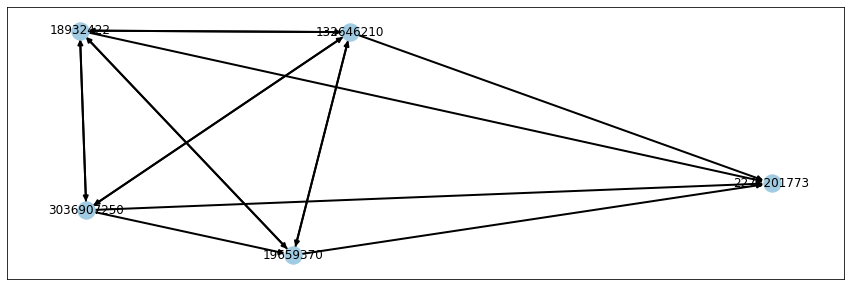
\includegraphics[scale=0.4]{images/max clique.png} %[width=.8\textwidth, height=.6\textheight, keepaspectratio]
    \label{fig:cricca_max}
\end{figure}


\subsection{Calcolo della copertura minima}
Si ricava l’albero di copertura minima (sempre sull’ego-grafo già ricavato) attraverso la funzione nx.min\_edge\_cover. 


\subsection{Stima della “small-world-ness” del grafo}
Lo ”small-world-ness effect” (“effetto piccolo mondo”) è un fenomeno che si può osservare all’interno di una rete nella quale i nodi sono strettamente connessi tra di loro e le distanze dei percorsi che li interconnettono sono relativamente brevi. \\* \\*
Per misurare l'effetto, si ricavano e si analizzano i coefficienti Omega e Sigma (per ricavare, si eseguono i metodi nx.omega ed nx.sigma sul grafo indiretto). Si veda la documentazione di Networkx per vedere come vengono calcolati:
\begin{itemize}
    \item Il risultato previsto per Omega è un valore compreso tra 1 e -1; se vicino allo zero significa che si ha small-world-ness. Nel nostro caso, si ricava il valore 0.0029;
    \item Per Sigma invece, si dice che si ha small-world-ness se è > 1. Nel nostro caso, si ricava il valore 0.94, che non è propriamente > 1, ma si avvicina molto.
\end{itemize}
Considerando i risultati osservati per Sigma e Omega, si può affermare che nella rete analizzata si verifica l’effetto piccolo mondo.



% -------------------------------------------------------------------------------- %
% ---------------------------------- CONCLUSIONI --------------------------------- %
% -------------------------------------------------------------------------------- %

\section{Bibliografia e sitografia}\label{sec:biblio_e_sito}
\begin{itemize}
    \item lezioni e slide del prof. Soprano Micheal (sito ufficiale: \url{https://michaelsoprano.com/})
    \item lezioni e slide del prof. Mizzaro Stefano (sito ufficiale: \url{http://users.dimi.uniud.it/~stefano.mizzaro/}) 
    \item documentazione ufficiale Tweepy: \url{http://docs.tweepy.org/en/latest/}
    \item documentazione ufficiale Networkx: \url{https://networkx.org/documentation/stable/index.html}
    \item documentazione ufficiale Pandas: \url{https://pandas.pydata.org/docs/}
    \item documentazione ufficiale PyVis: \url{https://pyvis.readthedocs.io/en/latest/}
\end{itemize}





\end{document}